\subsection{Present consequences and outcomes}

It is often the case the the data itself is not interesting to users in-and-of-itself.
Rather, what is relevant to the user are the consequences of the reality that the data indicates.
It is important to dedicate the necessary time to model such consequences, and the ways in which
those consequences impact the user. The points that should be made clear are: \\

\textbf{Objective}. Conceptually, what problems do we want to solve or clarify. It is very important that we have a clear objective,
     Even if we do not have prior expertise in the subject, having a well-defined objective helps us find the solution, or
     at least enables us to describe it more clearly to the expert who can solve the problem. \\

\textbf{Important points}. As mentioned earlier, our goal is not to show all the values, but
     rather to provide the user with important information in order to discover the significant consequences that can impact them, either positive or negative.

% TODO: don't understand this well enough to translate
% At a more technical level, it would be the limits or values of what data are those that provide us with information
% of an exceptional situation, or the values that we are trying to identify more easily. \\

\textbf{Data workflow}. When planning the flow of information, it must be clear how the data is transformed from data points to meaninful consequences and outcomes.

\subsubsection*{Suggested strategies} 

\begin{itemize}
    \item Once a goal has been set, we must stipulate the necessary fields of the dataset that we need. That is, we select the fields that interest us. 
    \item Analyze the data provided and see if the list of fields that the source offers us is sufficient to reach the chosen objective.
    If not directly, then via some derived process.
    \item Decide which values are more outstanding and provide them to the user.
\end{itemize}

\subsubsection*{In the context of Aire Guru \ldots}

Our main objective is to create awareness of the importance of air pollution in our health.
So we were not interested in the air pollution levels per se, but rather in showing how air pollution affects health.
To accomplish this we considered the following questions:

\begin{itemize}
    \item What diseases are affected by air pollution.
    \item What pollutants are those that create or influence diseases.
    \item What are the sources of each pollutant?.
    \item What is the representative measure of the level of air pollution.
    \item How it is calculated and what parameters we need for its calculation.
    \item What are the harmful levels in general and for each pollutant.
\end{itemize}

The measure that best represents the level of air pollution in this case is the AQI.
The city of Málaga is covered by the European legislation, so we focussed on official sources in this legislative region.
We looked for the relationships that pollutants have with different diseases.
For this we used clinical studies.
For each of the diseases, we researched the symptoms and how they can be aggravated by each pollutant.
For each pollutant, we looked for typical sources of pollution, to see if they occur in the city of Málaga and in what concentrations.
With all this information we determined that the pollutants that have common medical outcomes are \ch{CO}, \ch{NO2}, \ch{O3} and PM (Particulated Material).
Dfferent levels of particles affect different diseases in different ways.
We provide the information we used to justify our derived conclusions in the Glossary of Aire Guru. \\

Once these pollutants were selected, we determined if we have the appropriate data in our dataset.
As mentioned earlier, some samples show measurements from fixed and/or mobile stations and these can be quantitative or qualitative and others can be incomplete.
We have to select the samples to provide either the most complete information or the most accurate.
We prioritize quantitative measures over qualitative ones and in the case that there is only a qualitative measure, we map as follows:
Good $\rightarrow 50$, Acceptable $\rightarrow 150$, Poor $\rightarrow 300$, Bad $\rightarrow 400$, Unhealthy $\rightarrow 500$,
and we inform the user that the value is approximated.\\

At this point we know how air pollution affects our health.
We make very clear which are the undesirable values by using the alert colors, yellow, orange and red.
These colors are chosen in the palette of the colors provided by the EAQI.
In addition, the icon that represents unhealthy levels of pollution, is totally different, designed to clearly convey danger. \\

\begin{figure}[ht]
    \centering
    \subfigure[BarChart Aire Guru]
        {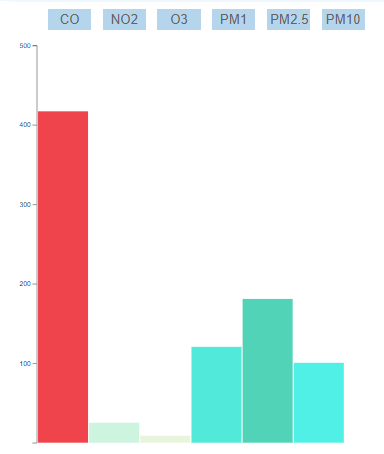
\includegraphics[width=5cm]{barchart}}
    \hfill
    \subfigure [Categoria medio ambiente]
        {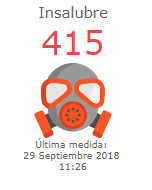
\includegraphics[width=4cm]{unhealthyIcon}}
    \caption{Alert situation}
\end{figure}

We guide the user from the selection of a point in the city of Málaga, either on their own initiative
or automatically, to the details of this point in real time and we continue to show the evolution of the pollution at that point.
The logic of this is that it is anticipated that the user will be interested in the pollution that surrounds them in real time and if
they want to know the breakdown of the pollutants at the point where they are, they can continue to inquire.
The map, in addition to showing the point where the user is, shows the user that the system is responsive.